\section{空间向量基本定理}

本节要点:
\begin{itemize}
    \item 掌握空间向量基本定理。
\end{itemize}

\begin{theorem}[空间向量基本定理]
设$\boldsymbol{a},\boldsymbol{b},\boldsymbol{c}$为三个不共面的空间向量,则对于任意向量$\boldsymbol{p}$,存在唯一的有序实数组$\left( x,y,z \right) $,使得
\[
\boldsymbol{p}=x\boldsymbol{a}+y\boldsymbol{b}+z\boldsymbol{c}
\]
我们把$\left\{ \boldsymbol{a},\boldsymbol{b},\boldsymbol{c} \right\} $称作空间的一个{\bf 基},把$\boldsymbol{a},\boldsymbol{b},\boldsymbol{c}$称作{\bf 基向量},对应的$\left( x,y,z \right) $称为$\boldsymbol{p}$在该组基下的{\bf 坐标}。
\end{theorem}

该定理和平面向量基本定理一样,指的是向量可以由基组合得到。也要注意,定理表达的意思是给定一个基就有一个坐标与之对应,所以不同的基有不同的坐标,但$\boldsymbol{p}$还是那个$\boldsymbol{p}$,也即:
\[
\boldsymbol{p}=x\boldsymbol{a}+y\boldsymbol{b}+z\boldsymbol{c}=l\boldsymbol{d}+m\boldsymbol{e}+n\boldsymbol{f}
\]

%============================================================
\subsection{习题}

\begin{example}[拓广探索8,难度:$\star \star $]
已知四面体中三组相对棱的中点间的距离都相等,求证:这个四面体相对的棱两两垂直。
\end{example}

解:

如下图,不难得到三组相对棱的中点连接的向量:

\begin{figure}[h]
\centering
\begin{minipage}{.32\textwidth}
\centering
\begin{tikzpicture}[style={x={(-135:0.5)},y={(1cm,0)},z={(0,1cm)}}, line join=round, scale=2.5]
\coordinate[label=left:      {$A$}] (A) at (0,-0.5,0);
\coordinate[label=below:     {$B$}] (B) at (0.7,0,0);
\coordinate[label=right:     {$C$}] (C) at (0,0.5,0);
\coordinate[label=above:     {$O$}] (O) at (0,0,0.7);
\coordinate[label=below left:{$D$}] (D) at ($(A)!0.5!(B)$);
\coordinate[label=right:     {$E$}] (E) at ($(O)!0.5!(C)$);
\draw[thick] (B)--(O)--(A)--(B)--(C)--(O);
\draw[dashed] (A)--(C);
\draw[dashed,red] (D)--(E) (O)--(D)--(C);
\end{tikzpicture}
\end{minipage}
\begin{minipage}{.32\textwidth}
\centering
\begin{tikzpicture}[style={x={(-135:0.5)},y={(1cm,0)},z={(0,1cm)}}, line join=round, scale=2.5]
\coordinate[label=left:       {$A$}]  (A) at (0,-0.5,0);
\coordinate[label=below:      {$B$}]  (B) at (0.7,0,0);
\coordinate[label=right:      {$C$}]  (C) at (0,0.5,0);
\coordinate[label=above:      {$O$}]  (O) at (0,0,0.7);
\coordinate[label=below right:{$D'$}] (D) at ($(A)!0.5!(C)$);
\coordinate[label=left:       {$E'$}] (E) at ($(O)!0.5!(B)$);
\draw[thick] (B)--(O)--(A)--(B)--(C)--(O);
\draw[dashed] (A)--(C);
\draw[dashed,red] (D)--(E) (O)--(D)--(B);
\end{tikzpicture}
\end{minipage}
\begin{minipage}{.32\textwidth}
\centering
\begin{tikzpicture}[style={x={(-135:0.5)},y={(1cm,0)},z={(0,1cm)}}, line join=round, scale=2.5]
\coordinate[label=left:       {$A$}]   (A) at (0,-0.5,0);
\coordinate[label=below:      {$B$}]   (B) at (0.7,0,0);
\coordinate[label=right:      {$C$}]   (C) at (0,0.5,0);
\coordinate[label=above:      {$O$}]   (O) at (0,0,0.7);
\coordinate[label=below right:{$D''$}] (D) at ($(B)!0.5!(C)$);
\coordinate[label=left:       {$E''$}] (E) at ($(O)!0.5!(A)$);
\draw[thick] (B)--(O)--(A)--(B)--(C)--(O);
\draw[dashed] (A)--(C);
\draw[dashed,red] (D)--(E) (O)--(D)--(A);
\end{tikzpicture}
\end{minipage}
\end{figure}

\begin{align*}
&\overrightarrow{DE}=-\frac{1}{4}\left( \overrightarrow{OB}+\overrightarrow{OA}+\overrightarrow{CB}+\overrightarrow{CA} \right) \\
&\overrightarrow{D'E'}=-\frac{1}{4}\left( \overrightarrow{OA}+\overrightarrow{OC}+\overrightarrow{BA}+\overrightarrow{BC} \right) \\
&\overrightarrow{D''E''}=-\frac{1}{4}\left( \overrightarrow{AB}+\overrightarrow{AC}+\overrightarrow{OB}+\overrightarrow{OC} \right)
\end{align*}
若要平方进行长度相等,非常复杂,我们简化,使之都用$OX$表示:
\begin{align*}
&\overrightarrow{DE}=-\frac{1}{2}\left( \overrightarrow{OB}+\overrightarrow{OA}-\overrightarrow{OC} \right) \\
&\overrightarrow{D'E'}=-\frac{1}{2}\left( \overrightarrow{OA}+\overrightarrow{OC}-\overrightarrow{OB} \right) \\
&\overrightarrow{D''E''}=-\frac{1}{2}\left( \overrightarrow{OB}+\overrightarrow{OC}-\overrightarrow{OA} \right)
\end{align*}
取$\left| \overrightarrow{DE} \right|=\left| \overrightarrow{D'E'} \right|$分析:
\begin{align*}
&\because \left| \overrightarrow{DE} \right|=\left| \overrightarrow{D'E'} \right| \\
&\therefore \left( \overrightarrow{OB}+\overrightarrow{OA}-\overrightarrow{OC} \right) ^2=\left( \overrightarrow{OA}+\overrightarrow{OC}-\overrightarrow{OB} \right) ^2 \\
&\therefore \overrightarrow{OB}\cdot \overrightarrow{OA}-\overrightarrow{OA}\cdot \overrightarrow{OC}=\overrightarrow{OA}\cdot \overrightarrow{OC}-\overrightarrow{OA}\cdot \overrightarrow{OB} \\
&\therefore \overrightarrow{OB}\cdot \overrightarrow{OA}-\overrightarrow{OA}\cdot \overrightarrow{OC}=0 \\
&\therefore \overrightarrow{OA}\cdot \left( \overrightarrow{OB}-\overrightarrow{OC} \right) =0 \\
&\therefore \overrightarrow{OA}\cdot \overrightarrow{CB}=0
\end{align*}
余下略。

深入分析:

结合上一节的拓广探索9,若三对棱垂直了,计算一下对棱的中点距。

\begin{figure}[h]
\centering
\begin{minipage}{.49\textwidth}
\centering
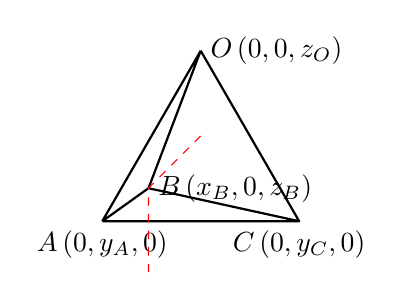
\begin{tikzpicture}[style={x={(-135:0.5)},y={(1cm,0)},z={(0,1cm)}}, line join=round, scale=2.5]
\mydrawxyz{0}{1.1}{-0.8}{0.8}{0}{1.1}
\coordinate[label=below:{$A\left( 0,y_A,0 \right) $}]   (A) at (0,-0.5,0);
\coordinate[label=below:{$C\left( 0,y_C,0 \right) $}]   (C) at (0,0.5,0);
\coordinate[label=right:{$B\left( x_B,0,z_B \right) $}] (B) at (0.75,0,0.433);
\coordinate[label=right:{$O\left( 0,0,z_O \right) $}]   (O) at (0,0,0.866);
\coordinate (Bx) at (0.75,0,0);
\coordinate (Bz) at (0,0,0.433);
\draw[thick] (O)--(A) (O)--(B) (O)--(C) (A)--(B)--(C)--(A);
\draw[dashed,red] (Bz)--(B)--(Bx);
\end{tikzpicture}
\end{minipage}
\begin{minipage}{.49\textwidth}
\centering
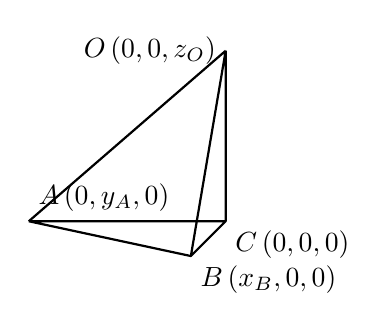
\begin{tikzpicture}[style={x={(-135:0.5)},y={(1cm,0)},z={(0,1cm)}}, line join=round, scale=2.5]
\mydrawxyz{0}{1.1}{-1.3}{0.3}{0}{1.1}
\coordinate[label=above right:{$A\left( 0,y_A,0 \right) $}] (A) at (0,-1,0);
\coordinate[label=below right:{$C\left( 0,0,0 \right) $}]   (C) at (0,0,0);
\coordinate[label=below right:{$B\left( x_B,0,0 \right) $}] (B) at (0.5,0,0);
\coordinate[label=left:       {$O\left( 0,0,z_O \right) $}] (O) at (0,0,0.866);
\draw[thick] (O)--(A) (O)--(B) (O)--(C) (A)--(B)--(C)--(A);
\end{tikzpicture}
\end{minipage}
\end{figure}

以$OA,BC$为例,它们的中点距为$\left( \frac{x_B}{2},\frac{y_A}{2},\frac{z_B}{2} \right) ,\left( 0,\frac{y_C}{2},\frac{z_O}{2} \right) $的距离,令$l$,则有:
\begin{align*}
&\because OA\bot BC\Rightarrow \left( 0,y_A,-z_O \right) \cdot \left( -x_B,y_C,-z_B \right) =0 \\
&\therefore y_Ay_C+z_Oz_B=0 \\
&\therefore l^2=\left( \frac{x_B}{2} \right) ^2+\left( \frac{y_A-y_C}{2} \right) ^2+\left( \frac{z_B-z_O}{2} \right) ^2 \\
&\therefore 4l^2={x_B}^2+{y_A}^2+{y_C}^2+{z_B}^2+{z_O}^2=OA^2+BC^2
\end{align*}
而且有:
\[
OA^2+BC^2=OC^2+AB^2=OB^2+AC^2
\]
这也是对棱垂直的四面体的性质,不难发现,正四面体和长方体一角都是该式的特殊形式。

\begin{tcolorbox}
本题思路简单,从定义出发,但是计算量大,如果不将一开始的表达式化简,几乎无解。
\end{tcolorbox}




